\chapter{Debugger}
\label{chap:debugger}
In diesem Kapitel wird beschrieben, wie der Debugger in Eclipse integriert wurde. Es wird aufgezeigt, was für Möglichkeiten existieren einen Debugger in Eclipse zu integrieren und welche implementiert wurden.

\section{Breakpoints}
Als erstes müssen für den Debugger Breakpoints gesetzt werden können. Dafür stehen zwei Möglichkeiten zur Verfügung, welche in den nächsten Kapiteln erläutert und verglichen werden.

\subsection{Per Konsole}

Die erste Möglichkeit ist, die Breakpoints per Konsole zu setzen. Das senden der Commands funktioniert mit den im Kapitel \ref{forthcommunication} beschriebenen Klassen. In der Konsole kann der Command

%
\begin{verbatim}
debug _function
\end{verbatim}
%
abgesetzt werden, um einen Breakpoint zu setzen.

\subsection{Im Source Code}

Eine weitere Möglichkeit ist, Breakpoints im C-File zu setzen. Dies wurde so umgesetzt, dass der Breakpoint nur auf eine Funktionsdefinition gesetzt werden kann. Alle anderen Zeilen des C-Source Codes können nicht direkt auf den übersetzten Forth Code abgebildet werden und sind deshalb nicht erlaubt für die Breakpoints.
\newline
Eclipse CDT stellt den Abstract Synatx Tree (AST) des C-Files zur Verfügung. Mit Hilfe des AST kann überprüft werden, ob sich der Breakpoint wirklich auf einer Funktionsdefinition befindet.
\newpage
\section{Konsolen basierter Debugger}

Eine eifache Integration des Debuggers ist, den schon existierenden Forth Konsolen Debugger im Eclipse zu verwenden. Dieser kann mit dem im Kapitel \ref{forthcommunication} beschriebenen Prozess Kommunikationsmitteln angesteuert und in einer Eclipse Console View angezeigt werden.

\begin{figure}[H]
	\centering
		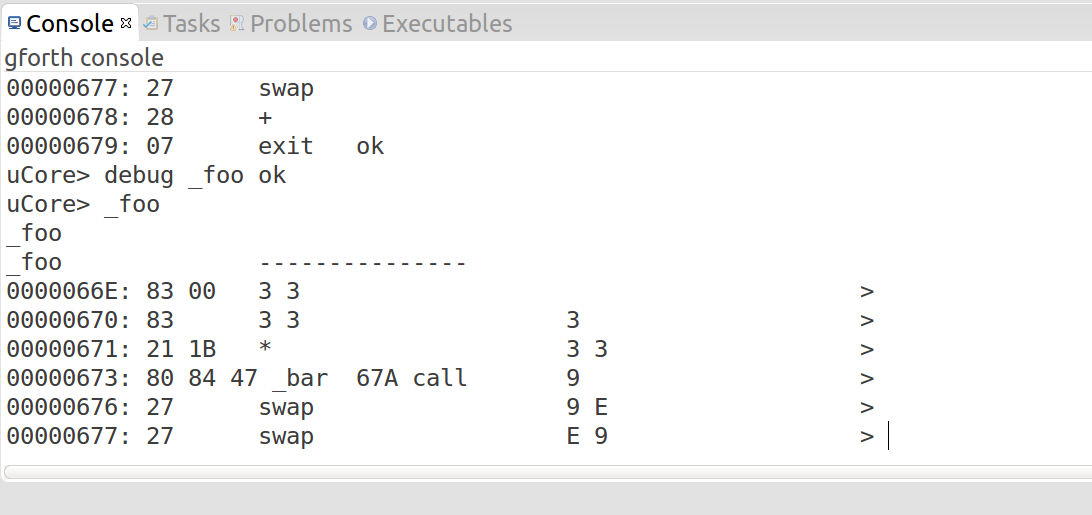
\includegraphics[scale=0.35]{debugger/consoledebugger.png}
		\caption{Konsolen basierter Debugger. Der Debugger kann über die Eclipse Console View gesteuert werden.}
		\captionsetup{margin=0cm,font={footnotesize}}
		\label{fig:consoledebugger}
\end{figure}

\section{Forth Debugger}

Eine weiter Möglichkeit ist, das Debug User Interface von Eclipse zu verwenden um den Debugger zu steuern. Dies ist für den Endanwender angenehmer, da  alle Informationen des Debuggers in einem User Interface ersichtlich sind.

\subsection{CDT oder JDT Debuggint Mechanismen}

Das Eclipse JDT stellt  mehrere Möglichkeiten zur Verfügung, wie ein Debugger integriert werden kann. Es können die vom Eclipse JDT verwendeten Mechanismen (vorallem das Plugin org.eclipse.debug.core), oder die vom CDT erweiterten Mechanismen (vorallem das Plugin org.eclipse.cdt.debug.core), welche verwendet werden um einen C oder C++ Debugger zu integrieren. Das vom CDT zur Verfügung gestellte Plugin wird vorallem dazu verwendet, um ein neuer C oder C++ Debugger zu integrieren, da es sich aber um einen Forth Debugger handelt, werden diese Erweiterungen nicht gebraucht. Ich habe mich deshalb dazu entschieden, das JDT Debugging zu verwenden.

\subsection{Debugger Aktionen}

Für den Debugger wurden einige Aktionen, welche schon im Eclipse verwendet werden, implementiert und einige neue Forth spezifische Aktionen hinzugefügt.

\subsubsection{Resume}

Mit der Resume Aktion kann der während dem Debuggen fortgeführt werden. Dafür wird ein \verb! end-trace! Command an den Forth Prozess gesendet. Der \verb! end-trace! Command entfernt auch alle Breakpoints, diese werden automatisch nach der Ausführung neu gesetzt. 

\begin{figure}[H]
	\centering
		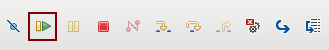
\includegraphics[scale=1]{debugger/resume.png}
		\caption{Resume Aktion.}
		\captionsetup{margin=0cm,font={footnotesize}}
		\label{fig:resume}
\end{figure}

\subsubsection{Terminate}

Mit der Terminate Aktion kann der Prozess heruntergefahren werden, in dem der \verb! bye! Command gesendet wird. Falls der Prozess nicht mehr reagiert, sollte die Kill Aktion verwendet werden. Die Terminate Aktion unterscheidet sich von der Kill Aktion, in dem sie versucht den Prozess auf normale Weise zu beenden und nicht über ein Kill Signal.

\begin{figure}[H]
	\centering
		
\includegraphics[scale=1]{debugger/terminate.png}
		\caption{Terminate Aktion.}
		\captionsetup{margin=0cm,font={footnotesize}}
		\label{fig:terminate}
\end{figure}

\subsubsection{Step Into}

Mit der Step Into Aktion kann in eine Funktion gesprungen werden, falls die nächste Zeile ein Funktionsaufruf ist. Dafür wird ein \verb! nest! Command an den Forth Prozess gesendet.

\begin{figure}[H]
	\centering
		
\includegraphics[scale=1]{debugger/stepinto.png}
		\caption{Step Into Aktion.}
		\captionsetup{margin=0cm,font={footnotesize}}
		\label{fig:stepinto}
\end{figure}

\newpage

\subsubsection{Step}

Mit der Step Aktion kann ein normaler single step ausgeführt werden. Dafür wird ein \verb! CR! Command an den Forth Prozess gesendet.

\begin{figure}[H]
	\centering
		
\includegraphics[scale=1]{debugger/step.png}
		\caption{Step Aktion.}
		\captionsetup{margin=0cm,font={footnotesize}}
		\label{fig:step}
\end{figure}

\subsubsection{Kill}

Mit der Kill Aktion kann der Prozess terminiert werden, in dem das Kill Signal gesendet wird. Im Normalfall sollte die Terminate Aktion verwendet werden, da sie den Forth Prozess über den \verb! bye! Command beendet.

\begin{figure}[H]
	\centering
		
\includegraphics[scale=1]{debugger/kill.png}
		\caption{Kill Aktion.}
		\captionsetup{margin=0cm,font={footnotesize}}
		\label{fig:kill}
\end{figure}

\subsubsection{After}

Die After Aktion setzt den Breakpoint nach der nächsten Instruktion, falls es sich um einen Rückwärts Sprung handelt, welcher möglicherweise von einer 
\verb! UNTIL!, \verb! REPEAT!, \verb! LOOP! oder \verb! NEXT! Instruktion kompiliert wurde. Der Rest der Schleife wird deshalb ohne Unterbruch ausgeführt.

\begin{figure}[H]
	\centering
		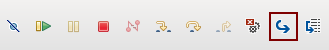
\includegraphics[scale=1]{debugger/after.png}
		\caption{After Aktion.}
		\captionsetup{margin=0cm,font={footnotesize}}
		\label{fig:after}
\end{figure}

\subsubsection{Jump}

Mit der Jump Aktion kann über die nächste auszuführende Instruktion gesprungen werden. Dafür wird ein \verb! jump! Command an den Forth Prozess gesendet.

\begin{figure}[H]
	\centering
		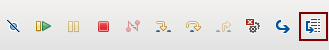
\includegraphics[scale=1]{debugger/jump.png}
		\caption{Jump Aktion.}
		\captionsetup{margin=0cm,font={footnotesize}}
		\label{fig:jump}
\end{figure}

\newpage

\subsection{Stack View}

In der Stack View wird er aktuelle Data-Stack angezeigt. Die Stack View wird automatisch nach jedem steppen des Debuggers aktualisiert.

\begin{figure}[H]
	\centering
		
\includegraphics[scale=0.35]{debugger/stack.png}
		\caption{Stack View mit aktuellem Dstack Inhalt. Der Top Of Stack (TOS) ist zuoberst in der Liste.}
		\captionsetup{margin=0cm,font={footnotesize}}
		\label{fig:stack}
\end{figure}


\subsection{Memory View}

In der Memory View kann ein Memory Dump, welcher mit dem \verb!dump! Befehl von uForth abgefragt werden kann, angezeigt werden. Der Memory Dump wird automatisch nach jedem steppen des Debuggers aktualisiert.

\begin{figure}[H]
	\centering
		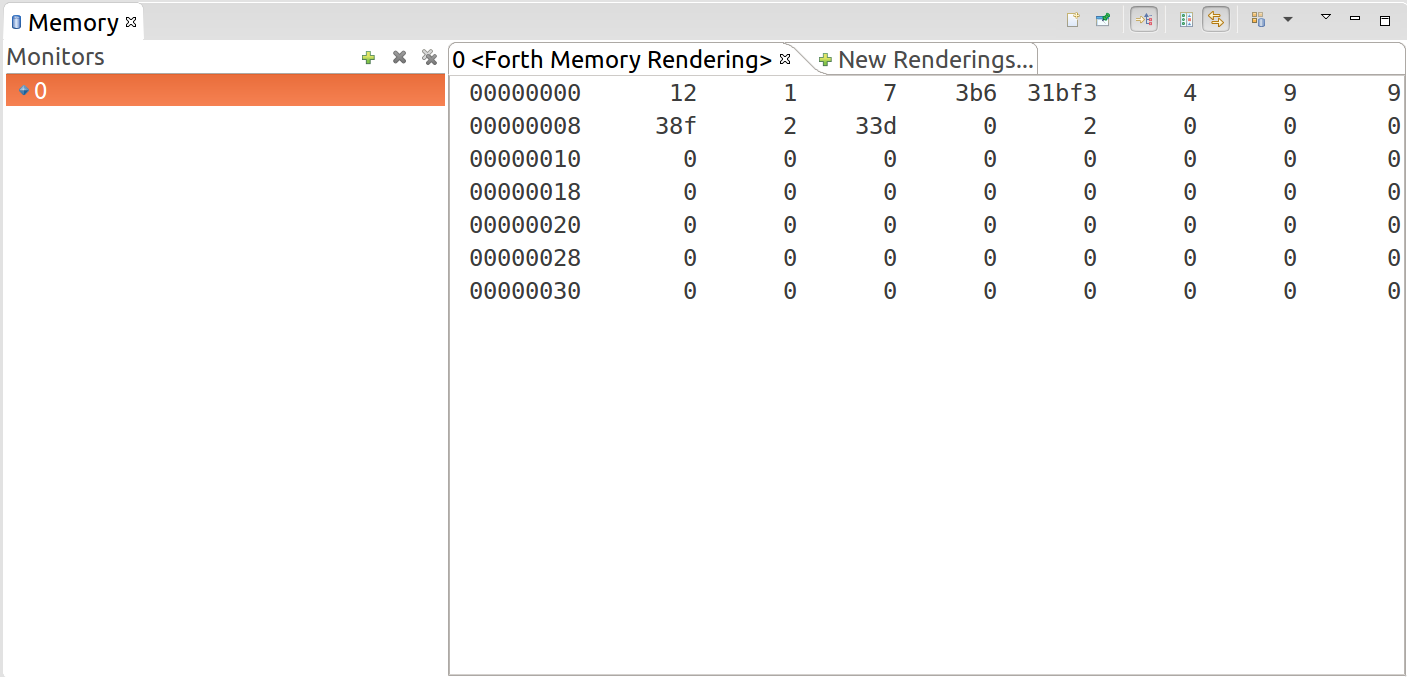
\includegraphics[scale=0.35]{debugger/dump.png}
		\caption{Eine Memory Dump, welcher}
		\captionsetup{margin=0cm,font={footnotesize}}
		\label{fig:dump}
\end{figure}


\section{C-Debugger}

Eine mögliche Erweiterung, wäre den Debugger so zu integrieren, das er direkt auf dem C-Source Code arbeitet (nicht wie bis jetzt, auf dem generierten Forth Code). Dies konnte nicht umgesetzt werden, da Debug Informationen des Compilers fehlen. Der C-Source Code kann nicht auf den entsprechenden generierten Forth Source Code abgebildet werden.